\section{Object 10}
\markright{Object 10}

The geometry of this object was achieved using the Revolved Boss/Base tool. The process began with the creation of a detailed 2D sketch representing the part's profile. This sketch was then revolved around a central axis. This method is highly efficient for such axisymmetric parts, generating the complex form from a single profile sketch.

\begin{figure}[H]
	\centering

	\begin{subfigure}[b]{0.49\textwidth}
		\centering
		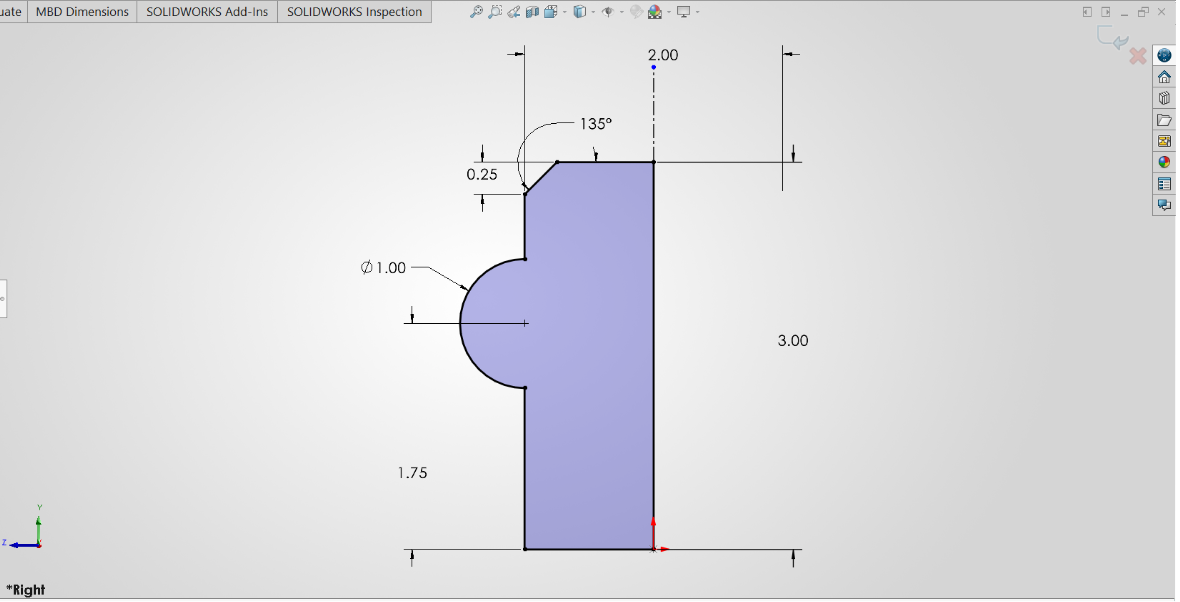
\includegraphics[width=\textwidth, keepaspectratio]{lab-01/assets/object-10/object-10-snap-1.png}
		\caption{2D sketch with dimensions}
	\end{subfigure}%
	\hfill
	\begin{subfigure}[b]{0.49\textwidth}
		\centering
		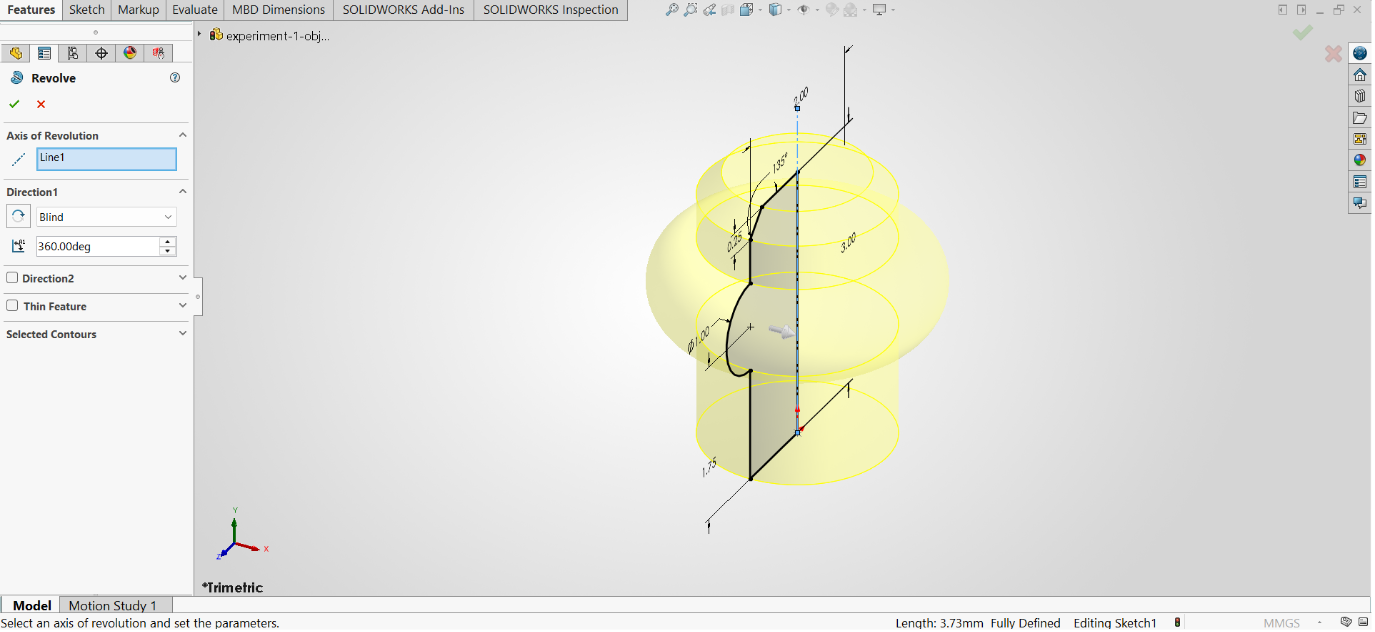
\includegraphics[width=\textwidth, keepaspectratio]{lab-01/assets/object-10/object-10-snap-2.png}
		\caption{Revolving the sketch around the vertical axis}
	\end{subfigure}%
	\vspace{0.5em}
	\begin{subfigure}[b]{\textwidth}
		\centering
		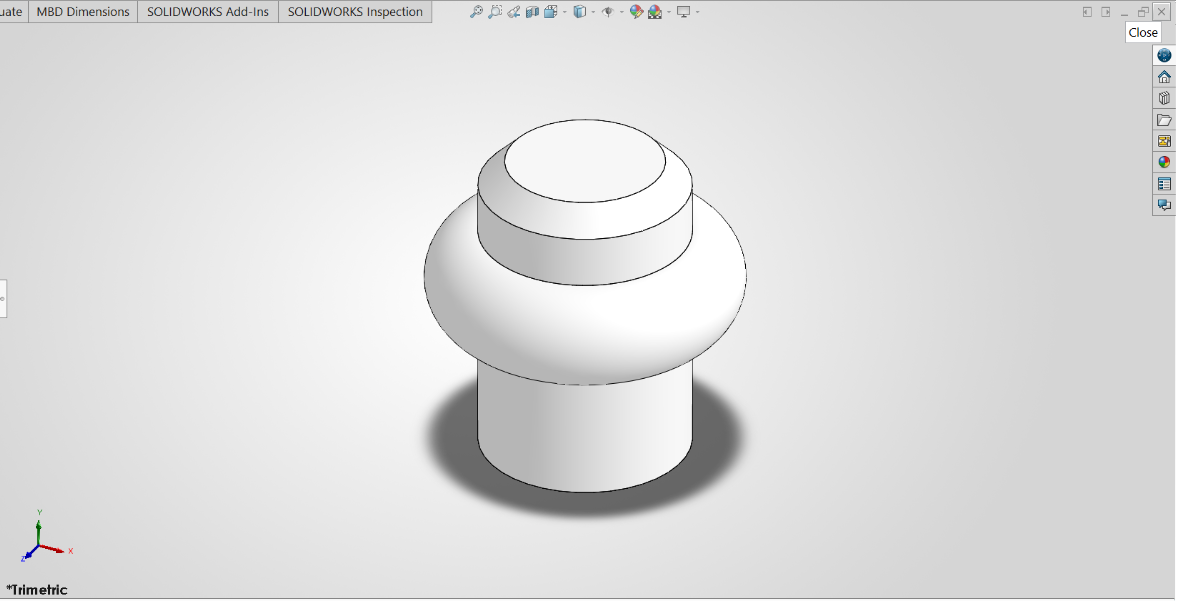
\includegraphics[width=\textwidth, keepaspectratio]{lab-01/assets/object-10/object-10-snap-3.png}
		\caption{Final Result}
	\end{subfigure}

	\caption{Snapshots while Designing Object 10 in Solidworks}
	\label{lab01_object_10}
\end{figure}
